\lstset{
style=python,
morekeywords={[2]
find,
index,
count,
split,
replace,
translate,
center,
rjust,
lower,
upper,
capitalize,
append,
insert,
pop,
reverse,
sort,
remove,
keys,
union,
intersection,
issubset,
add,
get,
values,
items,
}
}

\section{Wbudowane typy danych}\label{sec:data_types}
\begin{frame}{Wbudowane funkcje}
    \Wider{
    \begin{table}
        \centering
        \begin{tabular}{|l|l|}
            \hline
            print() & wypisanie na standardowe wyjście \\
            input() & pobranie ze standardowego wejścia \\
            \hline
            type() & typ zmiennej \\
            \hline
            range() & iterator sekwencji od a do b \\
            \hline
            abs() & wartość bezwzględna \\
            \hline
            min() & najmniejsza wartość sekwencji \\
            max() & największa wartość sekwencji \\
            \hline
            filter() & filtrowanie funkcyjne \\
            map() & mapowanie funkcyjne \\
            \hline
            reversed() & zwrócenie odwróconej sekwencji \\
            sorted() & zwrócenie posortowanej sekwencji \\
            \hline
            $\cdots$ & $\cdots$ \\
            \hline
        \end{tabular}
    \end{table}
    }
    \url{https://docs.python.org/3.7/library/functions.html} - wszystkie dostępne
\end{frame}

\begin{frame}{Typy danych}
    W Pythonie mamy wiele wbudowanych typów danych:
    \begin{itemize}
        \item float() - reprezentuje liczby rzeczywiste \footnote{Nie jest to do końca prawda, o czym przekonasz się na kolejnych slajdach.} \\
        \item int() - reprezentuje liczby całkowite \\
        \item str() - reprezentuje napisy - łańcuchy znaków \\
        \item bool() - reprezentuje wartości logiczne \\
        \item complex() - reprezentuje liczby urojone \\
        \item list() - reprezentuje zmienną grupę danych \\
        \item tuple() - reprezentuje uporządkowaną strukturę danych \\
        \item dict() - reprezentuje grupę danych, które da się indeksować \\
        \item set() - reprezentuje zbiór danych w rozumieniu teorii zbiorów \\
    \end{itemize}
    \url{https://docs.python.org/3.7/library/stdtypes.html} - wszystkie dostępne
\end{frame}

\begin{frame}{Klasyfikacja typów danych}
    \begin{columns}
        \begin{column}{0.5\textwidth}
            Typy skalarne:
            \begin{itemize}
                \item float() \\
                \item int() \\
                \item bool() \\
                \item str() - jako znak np. dla funkcji ord() \\
            \end{itemize}
            Typy drzewiaste:
            \begin{itemize}
                \item dict() \\
                \item set() \\
            \end{itemize}
            Typy liczbowe:
            \begin{itemize}
                \item float() \\
                \item int() \\
                \item complex() \\
            \end{itemize}            
        \end{column}
        \begin{column}{0.5\textwidth}
            Typy strukturalne:
            \begin{itemize}
                \item complex() \\
                \item str() - jako łańcuch znaków \\
                \item list() \\
                \item tuple() \\
                \item dict() \\
                \item set() \\
            \end{itemize}
            Typy sekwencyjne:
            \begin{itemize}
                \item str() - jako łańcuch znaków \\
                \item list() \\
                \item tuple() \\
            \end{itemize}
        \end{column}
    \end{columns}
\end{frame}

\begin{frame}{Przypisanie}
    \lstinputlisting{introduction/code/data_types/assignment.py}
\end{frame}


\section{Wbudowane skalarne typy danych}\label{sec:scalar_types}
\begin{frame}{Skalarne typy danych}
    \lstinputlisting{introduction/code/scalar_types/basic_types_1.py}
\end{frame}

\begin{frame}{Proste obliczenia}
    \lstinputlisting{introduction/code/scalar_types/basic_types_2.py}
\end{frame}

\begin{frame}{Operatory liczbowe - int, float}
    \begin{table}
        \centering
        \begin{tabular}{|c|l|}
            \hline
            $+$ & dodawanie \\
            \hline
            $-$ & odejmowanie \\
            \hline
            $*$ & mnożenie \\
            \hline
            $/$ & dzielenie \\
            \hline
            $**$ & potęgowanie \\
            \hline
            $//$ & dzielenie całkowitoliczbowe \\
            \hline
            $\%$ & reszta modulo \\
            \hline
        \end{tabular}
    \end{table}
\end{frame}

\begin{frame}{Obliczenia liczbowe - int, float}
    \lstinputlisting{introduction/code/scalar_types/numeral.py}
\end{frame}

\begin{frame}{Operacje binarne}
    NOT, $\lnot$, $\sim$ - negacja \\
    AND, $\land$ - koniunkcja \\
    NAND, $\barwedge$ - dysjunkcja \\
    OR, $\lor$ - alternatywa, suma logiczna, alternatywa zwykła, alternatywa nierozłączna, alternatywa łączna \\
    NOR, $\barvee$ - binegacja \\
    XOR, $\veebar$ - alternatywa rozłączna, alternatywa wykluczająca \\
    XNOR, $\iff$ - ekwiwalencja, równoważność \\
    IMPLY, $\implies$ - implikacja, wynikanie \\
    \scriptsize{
    \begin{table}
        \centering
        \begin{tabular}{|c|c||c|c||c|c||c|c||c|c||c|}
            \hline
            $p$ & $q$ & $\lnot p$ & $\sim q$ & $p \land q$ & $p \barwedge q$ & $p \lor q$ & $p \barvee q$ & $p \veebar q$ & $p \Leftrightarrow q$ & $p \Rightarrow q$ \\
            \hline
            F & F & T & T & F & T & F & T & F & T & T \\
            \hline
            F & T & T & F & F & T & T & F & T & F & T \\
            \hline
            T & F & F & T & F & T & T & F & T & F & F \\
            \hline
            T & T & F & F & T & F & T & F & F & T & T \\
            \hline
        \end{tabular}
    \end{table}
    }
\end{frame}

\begin{frame}{Operatory binarne - bool}
    \begin{table}
        \centering
        \begin{tabular}{|c|l|}
            \hline
            $<$ & mniejszy niż \\
            \hline
            $>$ & większy niż \\
            \hline
            $<=$ & mniejszy lub równy \\
            \hline
            $>=$ & większy lub równy \\
            \hline
            $==$ & równy \\
            \hline
            $!=$ & różny \\
            \hline
            $and$ & i \\
            \hline
            $or$ & lub \\
            \hline
            $not$ & negacja \\
            \hline
        \end{tabular}
    \end{table}
\end{frame}

\begin{frame}{Obliczenia binarne}
    \lstinputlisting{introduction/code/scalar_types/binary.py}
\end{frame}


\section{Wbudowane sekwencyjne struktury danych}\label{sec:sequence_types}
\begin{frame}{Struktura danych - lista}
    \begin{small}
        \begin{itemize}
            \item list() \\
            \item lista jednokierunkowa działa jak stos rezerwowy w grze pasjans - możemy
            podglądać jedną kartę i przesuwać się tylko do następnej \\
            \item lista dwukierunkowa pozwala przesuwać się w obie strony \\
            \item do listy możemy dodawać elementy w dowolne miejsce i usuwać je \\
            \item listy przyjaciół: [Ala, Ola, Ela] oraz [Ela, Ala, Ola] są równoważne - kolejność
            nie ma znaczenia \\
            \item jeśli powyższą listę potraktujemy jako posortowaną listę przyjaciół według jakiegoś
            kryterium, np. który z przyjaciół najlepiej gotuje, albo którą z przyjaciółek najchętniej
            zaproszę na studniówkę - wtedy kolejność będzie mieć znaczenie
        \end{itemize}
    \end{small}
    \begin{table}
        \centering
        \begin{tabular}{c|c|c|c|c|c|c}
            \cline{2-2} \cline{4-4} \cline{6-6}
            HEAD $\longrightarrow$ & DATA & \multirow{ 2}{*}{$\nearrow$} & DATA & \multirow{ 2}{*}{$\nearrow$} & DATA & \\
            \cline{2-2} \cline{4-4} \cline{6-6}
            & NEXT & & NEXT & & NEXT & $\longrightarrow$ NULL \\
            \cline{2-2} \cline{4-4} \cline{6-6}
        \end{tabular}
    \end{table}
\end{frame}

\begin{frame}{Struktura danych - krotka}
    \begin{itemize}
        \item tuple() \\
        \item para, trójka, czwórka, czyli ogólnie krotka \\
        \item uporządkowany rekord który ma niezmienną ilość i znaczenie pól \\
        \item np. (3, 4) jako współrzędne na płaszczyźnie - taką parę musimy interpretować
        w sposób (x=3, y=4) - nie możemy zamienić cyfr, w przeciwieństwie do listy znajomych
    \end{itemize}
\end{frame}

\begin{frame}{Operatory sekwencji}
    \begin{table}
        \centering
        \begin{tabular}{|c|l|}
            \hline
            $[]$ & dostęp przez indeks \\
            \hline
            $+$ & konkatenacja \\
            \hline
            $*$ & powtórzenie \\
            \hline
            $in$ & przynależność \\
            \hline
            $len$ & długość \\
            \hline
            $[::]$ & slicing \\
            \hline
        \end{tabular}
    \end{table}
\end{frame}

\begin{frame}{Operacje sekwencji}
    \lstinputlisting{introduction/code/sequence_types/sequence.py}
\end{frame}

\begin{frame}{Slicing}
    \lstinputlisting{introduction/code/sequence_types/slicing.py}
\end{frame}

\begin{frame}{Metody list}
    \Wider{
    \begin{table}
        \centering
        \begin{tabular}{|l|p{8cm}|}
            \hline
            alist.append(item) & dodanie na koniec listy \\
            \hline
            alist.insert(i,item) & wstawienie na konkretną pozycję na liście (dodawanie, nie zastępowanie) \\
            \hline
            alist.pop(i) & usunięcie i zwrócenie elementu z konkretnej (ostatniej) pozycji z listy \\
            \hline
            alist.sort() & posortowanie w miejscu (zmodyfikowanie) \\
            \hline
            alist.reverse() & odwrócenie w miejscu \\
            \hline
            del alist[i] & usunięcie elementu na pozycji bez zwracania - lepiej nie stosować \\
            \hline
            alist.index(item) & zwrócenie indeksu pierwszego wystąpienia w liście \\
            \hline
            alist.count(item) & zwrócenie liczby wystąpień w liście \\
            \hline
            alist.remove(item) & usunięcie pierwszego wystąpienia w liście \\
            \hline
        \end{tabular}
    \end{table}
    }
\end{frame}

\begin{frame}{Metody list}
    \begin{multicols}{2}
        \lstinputlisting[linewidth=0.4\textwidth]{introduction/code/sequence_types/lists.py}
    \end{multicols}
\end{frame}

\begin{frame}{Metody napisów}
    \Wider{
    \begin{table}
        \centering
        \begin{tabular}{|p{4cm}|p{7cm}|}
            \hline
            astring.center(s) & zwrócenie wyśrodkowanego napisu w polu o rozmiarze s (nie w miejscu) \\
            astring.ljust(s) & zwrócenie wyrównanego do lewej \\
            astring.rjust(s) & zwrócenie wyrównanego do prawej \\
            \hline
            astring.count(item) & zwrócenie liczby wystąpień podnapisu w napisie \\
            \hline
            astring.index(item) /\newline astring.find(item) & zwrócenie indeksu pierwszego wystąpienia podnapisu \\
            \hline
            astring.split(sep) & podzielenie napisu na listę napisów w miejscu wystąpienia podnapisów \\
            \hline
            astring.lower() & zamiana na małe litery \\
            astring.upper() & zamiana na duże litery \\
            astring.capitalize() & pierwsza duża, reszta mała \\
            \hline
            astring.replace(old, new) & zastąpienie podstringu nowym stringiem \\
            \hline
        \end{tabular}
    \end{table}
    }
\end{frame}

\begin{frame}{Metody napisów}
    \lstinputlisting{introduction/code/sequence_types/strings_1.py}
\end{frame}

\begin{frame}{Metody napisów}
    \lstinputlisting{introduction/code/sequence_types/strings_2.py}
\end{frame}

\begin{frame}{Metoda format()}
    \lstinputlisting{introduction/code/sequence_types/strings_format.py}
\end{frame}

\begin{frame}{Escape character, escape sequence}
    \begin{center}
        znak modyfikacji (escape character) = znak ucieczki = znak uwalniania \\
        sekwencja zmodyfikowana (escape sequence) = znak modyfikacji + sekwencja następująca \\
    \end{center}
    \lstinputlisting{introduction/code/sequence_types/strings_escape.py}
\end{frame}


\section{Wbudowane drzewiaste struktury danych}\label{sec:trees_types}
\begin{frame}{Struktura danych - słownik, mapa}
    \begin{itemize}
        \item dict() \\
        \item jest jak książka telefoniczna, znając klucz (nazwisko) możemy wyszukać wartość (numer telefonu) \\
        \item budowany z wykorzystaniem tablicy i funkcji skrótu(haszującej) - stąd jego inna nazwa - tablica
        z haszowaniem, mieszająca \\
        \item tablica ma tą przewagę nad listą, że dostęp do elementów mamy zapewniony w czasie stałym O(1),
        by pobrać element z listy musimy przejść po niej pesymistycznie w czasie liniowym O(n) \\
        \item lista ma tą przewagę nad tablicą, że nie musi przewidywać wielkości przyszłych danych - można
        ją dynamicznie poszerzać \\
        \item dzięki wykorzystaniu funkcji skrótu, możemy zmniejszyć rozmiar wymaganej tablicy \\
        \item alternatywnie może być zaimplementowany jako drzewo poszukiwań
    \end{itemize}
\end{frame}

\begin{frame}{Operatory słowników}
    \begin{table}
        \centering
        \begin{tabular}{|c|l|}
            \hline
            $[]$ & dostęp przez klucz \\
            \hline
            $in$ & przynależność \\
            \hline
            $del$ & usuwanie wartości pod kluczem \\
            \hline
        \end{tabular}
    \end{table}
\end{frame}

\begin{frame}{Metody słowników}
    \Wider{
    \begin{table}
        \centering
        \begin{tabular}{|l|l|}
            \hline
            adict.keys() & lista kluczy \\
            \hline
            adict.values() & lista wartości \\
            \hline
            adict.items() & lista par klucz-wartość \\
            \hline
            adict.get(k) & element pod kluczem \\
            adict.get(k,default) & element pod kluczem lub domyślny \\
            \hline
            adict.clear() & usunięcie wszystkich elementów ze słownika \\
            \hline
        \end{tabular}
    \end{table}
    }
\end{frame}

\begin{frame}{Metody słowników}
    \lstinputlisting{introduction/code/trees_types/dicts.py}
\end{frame}

\begin{frame}{Struktura danych - zbiór}
    \begin{itemize}
        \item set() \\
        \item zbiór danych w rozumieniu teorii zbiorów, czyli worek, do którego coś należy lub nie \\
        \item taki worek może być też wyobrażany jako słownik z tylko dwoma wartościami, True - gdy należy
        i False - gdy nie należy
    \end{itemize}
    Załóżmy że na kurs programowania chodzi 6 osób: \{Ala, Ela, Ola, Ula, Iza, Eberhard\}. \\
    Z rekurencją nie radzi sobie \{Ela, Ula\}. \\
    Metody HTTP są niezrozumiałe dla \{Ala, Ela, Iza\}. \\
    Algorytmów grafowych nie rozumieją \{Ela, Ola, Iza\}. \\
    Eberhard jako jedyny na zajęciach zadaje pytania, a w domu utrwala materiał - dlatego wszystko rozumie. \\
    Wymienione grupy osób są tematycznymi zbiorami, na których możemy wykonywać operację teoriomnogościowe:
    sumy, przecięcia, dopełnienia, itd.
\end{frame}

\begin{frame}{Operatory zbiorów}
    \begin{table}
        \centering
        \begin{tabular}{|c|l|}
            \hline
            $|$ & unia \\
            \hline
            $\&$ & intersekcja \\
            \hline
            $-$ & różnica \\
            \hline
            $<=$ & podzbiór \\
            \hline
            $in$ & przynależność \\
            \hline
            $len$ & liczność \\
            \hline
        \end{tabular}
    \end{table}
\end{frame}

\begin{frame}{Metody zbiorów}
    \Wider{
    \begin{table}
        \centering
        \begin{tabular}{|l|l|}
            \hline
            aset.union(otherset) & unia \\
            \hline
            aset.intersection(otherset) & intersekcja \\
            \hline
            aset.difference(otherset) & różnica \\
            \hline
            aset.issubset(otherset) & podzbiór \\
            \hline
            aset.add(item) & dodanie do zbioru \\
            \hline
            aset.remove(item) & usunięcie ze zbioru \\
            \hline
            aset.pop() & usunięcie kolejnego (losowego?) ze zbioru \\
            \hline
            aset.clear() & usunięcie wszystkich elementów ze zbioru \\
            \hline
        \end{tabular}
    \end{table}
    }
\end{frame}

\begin{frame}{Metody zbiorów}
    \lstinputlisting{introduction/code/trees_types/sets.py}
\end{frame}


\section{Instrukcje sterujące}\label{sec:controls}
\begin{frame}{If-Elif-Else}
    \lstinputlisting{introduction/code/controls/if_pattern.py}
    Konstrukcji \emph{if} używamy by wykonać pewny blok kodu wyłącznie, gdy spełniony jest warunek logiczny. Warunek musi wyrażać wartość logiczną. \\
    Konstrukcja \emph{elif} przydaje się, gdy chcemy sprawdzić sekwencyjnie kilka warunków logicznych. Jeśli którykolwiek zostanie spełniony, nie będziemy sprawdzać kolejnych warunków. \\
    Konstrukcja \emph{else} służy do zdefiniowania wszystkich pozostałych ścieżek, nie określonych w żadnym warunku.
\end{frame}

\begin{frame}{If-Elif-Else}
    \lstinputlisting{introduction/code/controls/if.py}
\end{frame}

\begin{frame}{While-Else}
    \lstinputlisting{introduction/code/controls/while_pattern.py}
    Konstrukcji \emph{while} używamy gdy chcemy powtarzać fragment kodu, \textbf{dopóki} jakiś warunek jest spełniony. Operacje zachodzące w ciele pętli powinny doprowadzić do sytuacji, w której warunek po skończonej liczbie kroków przestanie być spełniony. W przeciwnym wypadku utkniemy w pętli nieskończonej. \\
    Konstrukcja \emph{else} wykona się zawsze gdy warunek przyjmie wartość False, zarówno gdy od początku jest niespełniony (ciało pętli się nie wykona), jak również po wszystkich iterachach pętli (gdy warunek przestanie być spełniany). \textbf{Nie} wykona się, gdy z pętli wyszliśmy za pomocą słowa \emph{break}.
\end{frame}

\begin{frame}{While-Else}
    \lstinputlisting{introduction/code/controls/while.py}
\end{frame}

\begin{frame}{For-In-Else}
    \lstinputlisting{introduction/code/controls/for_pattern.py}
    Konstrukcji \emph{for ... in} używamy, gdy chcemy wykonać coś \textbf{dla każdej} wartości z jakiegoś zbioru (wyrażonego za pomocą iteratora). Iterować możemy po liście, krotce, zbiorze, napisie, itd. Funkcje wbudowane \emph{range()} oraz \emph{enumerate()} także zwracają iteratory. \\
    Konstrukcja \emph{else} działa na podobnej zasadzie, jak przy pętli \emph{while}. Ten blok kodu wykona się, gdy nie będzie już kolejnych wartości do iterowania (pętla wykonała się dla wszystkich, lub iterator od początku był pusty).
\end{frame}

\begin{frame}{For-In-Else}
    \lstinputlisting{introduction/code/controls/for.py}
\end{frame}

\begin{frame}{Break-Continue}
    \lstinputlisting{introduction/code/controls/break.py}
    Słowo kluczowe \emph{break} przerywa działanie najbardziej zagnieższonej pętli i przenosi sterowanie poza nią (\textbf{pomija} blok kodu w \emph{else}). \\
    Słowo kuczowe \emph{continue} przerywa wykonanie obecnej iteracji pętli i przechodzi do sprawdzenia warunku (\emph{while}), lub przechodzi do kolejnej wartości z iteratora (\emph{for}).
\end{frame}

\begin{frame}{Wyjątki}
    Wyjątek lub błąd (np. dzielenie przez zero, próba otwarcia nieistniejącego pliku) to sytuacja, w której działanie programu znalazło się w sytuacji, której nie można traktować jako poprawne wykonanie (happy path). \\
    Powoduje to przerwanie wykonania programu i eskalację błędu do najbliższego bloku kodu, który potrafi przechwycić ten wyjątek. Błąd eskaluje pokonując w odwrotnej kolejności stos wywołań i zagnieżdzeń funkcji. Jeśli wyjątek nie zostanie przechwycony, błąd eskaluje do najbardziej zewnętrznego wywołania i przerwie działanie programu. Jeśli wyjątek zostanie przechwycony, działanie programu zostanie wznowione w miejscu przechwycenia, a nie zgłoszenia wyjątku. \\
    Wyjątki nie powinny być wykorzystywane jako mechanizm standardowego przekazywania sterowania w programie - nie powinny zastępować warunków i pętli.
\end{frame}

\begin{frame}{Wyjątki - możliwości}
    \lstinputlisting{introduction/code/controls/exceptions_pattern.py}
\end{frame}

\begin{frame}{Wyjątki - możliwości}
   Słowo kluczowe \emph{raise} zgłasza wystąpienie wyjątku lub błędu. \\
   Konstrukcja \emph{try} definiuje blok kodu, wewnątrz którego spodziewamy się wystąpienia wyjątku. \\
   Konstrukcja \emph{except} pozwala przechwycić wyjątki konkretnych typów lub wszystkie wyjątki. W tym bloku kodu dokonujemy ich przetwarzania. \\
   Słowo kluczowe \emph{as} pozwala zapamiętać wyjątek w zmiennej i wykorzystać go w bloku \emph{except}. \\
   Konstrukcji \emph{else} używamy do zdefiniowania działań, które zostaną podjęte gdy żadny wyjątek nie zostanie zgłoszony. \\
   Konstrukcja \emph{finally} określa działania, które zostaną wykonane zawsze, nieważne, czy wyjątek został zgłoszony, czy nie (działa na podobnej zasadzie jak \emph{else} w przypadku pętli). W tym bloku zazwyczaj definiujemy działania sprzątające po kodzie wykonywanym w bloku \emph{try} (np. zamykanie plików).
\end{frame}

\begin{frame}{Wyjątki - bare except}
    Sposób na złapanie każdego wyjątku:
    \lstinputlisting[firstline=1, lastline=2]{introduction/code/controls/exceptions_bare_pattern.py}

    Sposób na złapanie każdego wyjątku i wykorzystanie danych które przenosi:
    \lstinputlisting[firstline=4, lastline=5]{introduction/code/controls/exceptions_bare_pattern.py}

    Sposób na ponowne zgłoszenie poprzedniego wyjątku - możemy wykonać jakieś operacje, np. zapisać treść błędu do logów, a następnie ponownie go zgłosić do dalszego przetwarzania:
    \lstinputlisting[firstline=7, lastline=9]{introduction/code/controls/exceptions_bare_pattern.py}
\end{frame}

\begin{frame}{Wyjątki}
    \lstinputlisting{introduction/code/controls/exceptions.py}
\end{frame}


\section{Funkcje}\label{sec:funcions}
\begin{frame}{Definicje funkcji}
    Dzięki zastosowaniu funkcji możemy reużywać fragmenty kodu oraz ukrywać szczegóły implementacyjne za interfejsem. \\
    Deklaracja funkcji (jej interfejs) to jej pierwsza linia (nazwa oraz przyjmowane parametry). Następujący po deklaracji blok kodu to definicja funkcji. \\
    Funkcja może być bezargumentowa lub przyjmować argumenty - ich skończoną lub nieskończoną liczbę. Skończona liczba argumentów może przyjmować wartości domyślne. \\
    Funkcja może zwracać jakąś wartość (słowo kluczowe \emph{return}) lub nie zwracać wartości. Funkcje generujące mogą zwracać wiele wartości (słowo kluczowe \emph{yield}). \\
    \begin{alertblock}{}
        Domyslne argumenty są ewaluowane tylko raz!
    \end{alertblock}
\end{frame}

\begin{frame}{Definicje funkcji}
    \lstinputlisting{introduction/code/functions/functions.py}
\end{frame}

\begin{frame}{Generatory}
    Generatory pozwalają leniwie generować po jednej wartości, bez konieczności przechowywania w pamięci wszystkich przyszłych wartości. \\
    \lstinputlisting{introduction/code/functions/generators.py}
\end{frame}

\begin{frame}{Gorliwy (eager) wujek}
    Funkcje mogą zwracać wartości leniwie lub gorliwie. Gorliwe funkcje od razu zwracają wszystkie wyniki, a leniwe zwracają po jednym za każdym razem gdy się je wywoła. \\
    \begin{exampleblock}{}
       Wujek Janusz jest gorliwy. Gdy proszę go o dowcip każe mi czekać i zapisuje wszystkie znane mu dowcipy na kartce, co trwa kilka godzin. Następnie wręcza mi kartkę i mówi, że gdy najdzie mnie ochota na dowcip, mogę po prostu przeczytać kolejny z kartki. Mam już w domu kilkanaście kartek pełnych tych samych dowcipów wujka Janusza. Taka lista przydała mi się gdy jechałen na kolonie i chciałem zabrać ze sobą wszystkie dowcipy. Czasem jednak chciałbym usłyszeć tylko jeden...
    \end{exampleblock}
\end{frame}

\begin{frame}{Leniwy (lazy) wujek}
    \begin{exampleblock}{}
        Wujek Stefan jest leniwy i zawsze gdy go poproszę opowiada tylko jeden dowcip. Kiedy chciałem spisać wszystkie jego dowcipy, żeby porównać ich listę z listą dowcipów wujka Janusza, musiałem wielokrotnie prosić go o kolejny dowcip i samemu je spisywać. Trwało to kilkanaście godzin, znacznie dłużej niż w przypadku wujka Janusza, który sam je zapisywał. Jednakże, gdy chcę usłyszeć tylko jeden dowcip, wujek Stefan jest znacznie lepszym wyborem niż wujek Janusz.
    \end{exampleblock}
    Generatory są leniwe i odpowiednio użyte mogą znacznie skrócić czas obliczeń. Użyte nieodpowiednio mogą go wydłużyć. \\
\end{frame}

\begin{frame}{Funkcje anonimowe}
    \lstinputlisting{introduction/code/functions/lambda.py}
\end{frame}


\section{Uzupełnienie}\label{sec:addons}
\begin{frame}{List, dict, set comprehension}
    \lstinputlisting{introduction/code/addons/comprehension.py}
\end{frame}

\begin{frame}{Płaski model pamięci}
    \begin{table}
        \centering
        \begin{tabular}{rc|c|}
            \cline{3-3}
            & & \\
            \cline{3-3}
            0x8000 & $\longrightarrow$ & $\cdots$ \\
            \cline{3-3}
            0x8001 & $\longrightarrow$ & 01110010 \\
            \cline{3-3}
            0x8002 & $\longrightarrow$ & 10010101 \\
            \cline{3-3}
            0x8003 & $\longrightarrow$ & 11011011 \\
            \cline{3-3}
            0x8004 & $\longrightarrow$ & 10111011 \\
            \cline{3-3}
            0x8005 & $\longrightarrow$ & 11110010 \\
            \cline{3-3}
            0x8006 & $\longrightarrow$ & 01110001 \\
            \cline{3-3}
            0x8007 & $\longrightarrow$ & 10110011 \\
            \cline{3-3}
            0x8008 & $\longrightarrow$ & 00101100 \\
            \cline{3-3}
            0x8009 & $\longrightarrow$ & $\cdots$ \\
            \cline{3-3}
            & & \\
            \cline{3-3}
        \end{tabular}
    \end{table}
\end{frame}

\begin{frame}{Przypisanie w pamięci}
    \begin{columns}
        \begin{column}{0.4\textwidth}
            \lstinputlisting{introduction/code/addons/memory_assignment_1.py}
            \begin{table}
                \centering
                \begin{tabular}{rc|c|}
                    \cline{3-3}
                    a & $\longrightarrow$ & 1 \\
                    \cline{3-3}
                    \\
                    \cline{3-3}
                    ? & $\longrightarrow$ & 1 \\
                    \cline{3-3}
                    a & $\longrightarrow$ & 2 \\
                    \cline{3-3}
                \end{tabular}
            \end{table}
        \end{column}
        \begin{column}{0.4\textwidth}
            \lstinputlisting{introduction/code/addons/memory_assignment_2.py}
            \begin{table}
                \centering
                \begin{tabular}{rc|c|}
                    \cline{3-3}
                    a & $\longrightarrow$ & 1 \\
                    \cline{3-3}
                    b & \multicolumn{1}{c}{$\nearrow$} & \multicolumn{1}{c}{} \\
                    \\
                    \cline{3-3}
                    a & $\longrightarrow$ & 2 \\
                    \cline{3-3}
                \end{tabular}
            \end{table}
        \end{column}
    \end{columns}
\end{frame}

\begin{frame}{Listy w pamięci}
    W wielu miejscach w pythonie korzystamy z referencji (wskaźników). W liście nie trzymamy wartości zmiennych, a wskaźniki na miejsca w których wartości zmiennych się znajdują. Dlatego mnożąc listę, mnożymy wskaźniki, a nie wartości. Następnie zmieniamy wartość na którą wskazuje wskaźnik, a nie sam wskaźnik.
    \lstinputlisting{introduction/code/addons/memory_assignment_3.py}
\end{frame}

\begin{frame}{Zmienne zmienne i niezmienne}
    Wartości zmiennych (variable) mogą być zmienne, mutowalne (mutable) lub niezmienne, niemutowalne (immutable). \\
    Wartości mutowalne mogą zmieniać swoją wartość w trakcie trwania programu. \\
    Wartości niemutowalne nie mogą się zmieniać - trzeba stworzyć nową wartość zmieniając część z jej części składowych. \\
    \lstinputlisting{introduction/code/addons/mutable.py}
\end{frame}

\begin{frame}{Ułamki}
    \begin{justify}
        Zauważmy, że:
        \begin{itemize}
            \item Każdy ułamek dziesiętny skończony lub nieskończony okresowy można zamienić w ułamek zwykły.
            Jedynie ułamka dziesiętnego nieskończonego nieokresowego nie da się zamienić. \\
            \item Każdy ułamek zwykły nieskracalny o mianowniku, będącym dzielnikiem
            jakiejś potęgi liczby 10 da się zamienić w ułamek dziesiętny skończony. \\
            \item Każdy ułamek zwykły nieskracalny o mianowniku niemającym tej własności
            jest równy pewnemu ułamkowi dziesiętnemu nieskończonemu okresowemu. \\
        \end{itemize}

        Ponieważ każdy ułamek zwykły to iloraz dwóch liczb całkowitych, więc każdy ułamek dziesiętny
        skończony lub nieskończony okresowy da się zapisać w postaci dwóch liczb całkowitych.
    \end{justify}
\end{frame}
\begin{frame}{Przeliczanie ułamków okresowych na zwykłe}
    \begin{gather*}
        0,(1234) = x | * 10000 \\
        1234,(1234) = 10000x \\
        1234,(1234) = 1234 + x \\
        1234 = 9999x \\
        x = \frac{1234}{9999} \\
        0,(1234) = \frac{1234}{9999} \\
    \end{gather*}
\end{frame}

\begin{frame}{Liczby rzeczywiste}
    Każda liczba rzeczywista jest jakimś ułamkiem dziesiętnym(również nieskończonym nieokresowym).

    Komputer jest maszyną skończoną i jako taki ma ograniczone zasoby. Z tego powodu w komputerze
    nie może przechowywać dokładnie niektórych rodzajów danych. Przykładem są liczby rzeczywiste,
    których jest nieskończenie wiele i których większość posiada nieskończone rozwinięcia dziesiętne.

    Rozpatrzmy liczbę $\pi$, która pozwoli nam lepiej zrozumieć problem.
    Poniżej przedstawiam jedynie pierwszych 1500 cyfr po przecinku jej rozwinięcia dziesiętnego.

\end{frame}
\begin{frame}{Pi, czyli 3,\dots}
    \centering
    14159265358979323846264338327950288419716939937510
    58209749445923078164062862089986280348253421170679
    82148086513282306647093844609550582231725359408128
    48111745028410270193852110555964462294895493038196
    44288109756659334461284756482337867831652712019091
    45648566923460348610454326648213393607260249141273
    72458700660631558817488152092096282925409171536436
    78925903600113305305488204665213841469519415116094
    33057270365759591953092186117381932611793105118548
    07446237996274956735188575272489122793818301194912
    98336733624406566430860213949463952247371907021798
    60943702770539217176293176752384674818467669405132
    00056812714526356082778577134275778960917363717872
    14684409012249534301465495853710507922796892589235
    42019956112129021960864034418159813629774771309960
\end{frame}
\begin{frame}{Pi, a dalej \dots}
    \centering
    51870721134999999837297804995105973173281609631859
    50244594553469083026425223082533446850352619311881
    71010003137838752886587533208381420617177669147303
    59825349042875546873115956286388235378759375195778
    18577805321712268066130019278766111959092164201989
    38095257201065485863278865936153381827968230301952
    03530185296899577362259941389124972177528347913151
    55748572424541506959508295331168617278558890750983
    81754637464939319255060400927701671139009848824012
    85836160356370766010471018194295559619894676783744
    94482553797747268471040475346462080466842590694912
    93313677028989152104752162056966024058038150193511
    25338243003558764024749647326391419927260426992279
    67823547816360093417216412199245863150302861829745
    55706749838505494588586926995690927210797509302955
\end{frame}
\begin{frame}{Liczby zmiennoprzecinkowe}
    Automat skończony jakim jest komputer nie mamy możliwości reprezentowania wszystkich liczb
    rzeczywistych, a jedynie ich mniej lub bardziej dokładne przybliżenia - mówi się, że float
    reprezentuje liczby zmiennoprzecinkowe, ponieważ w pamięci trzymane są w postaci znormalizowanej
    (czyli z przesuniętym przecinkiem) jako mantysa i wykładnik\footnote{zgodnie ze standardem IEEE 754}.
    \begin{center}
        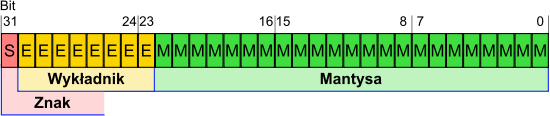
\includegraphics[width=0.7\textwidth]{introduction/graphics/ieee_full.png}
    \end{center}
\end{frame}

\begin{frame}{Przeliczanie liczb zmiennoprzecinkowych}
    \begin{center}
        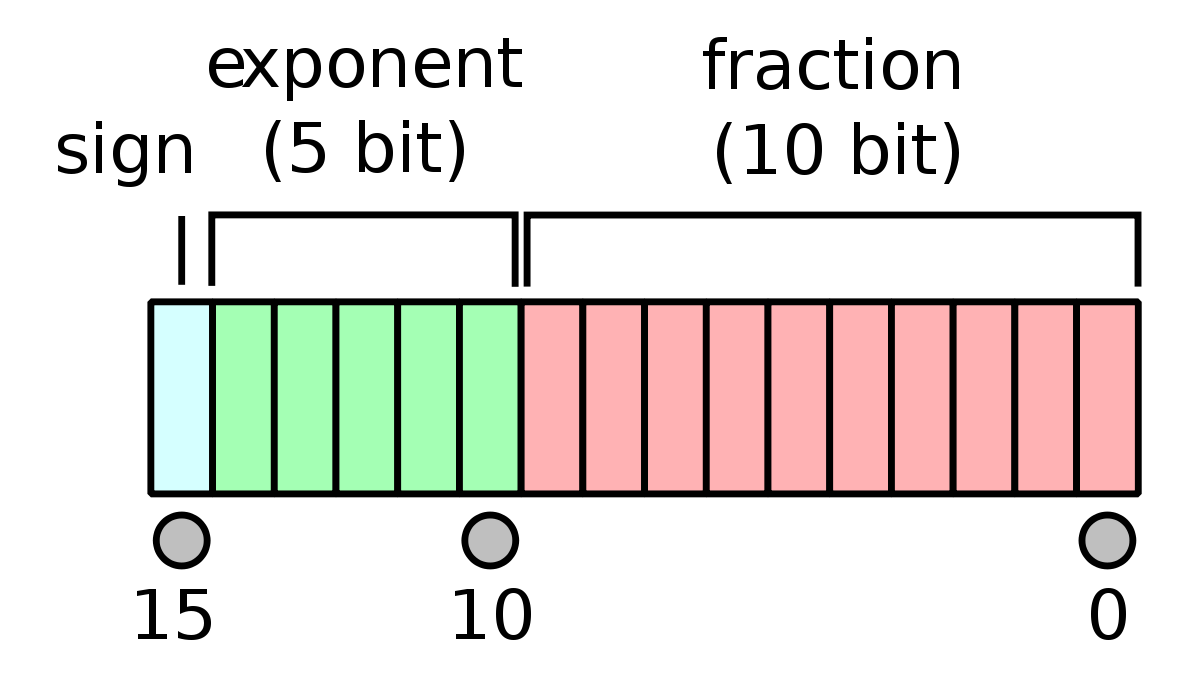
\includegraphics[height=0.2\textheight]{introduction/graphics/ieee_half.png} \\
        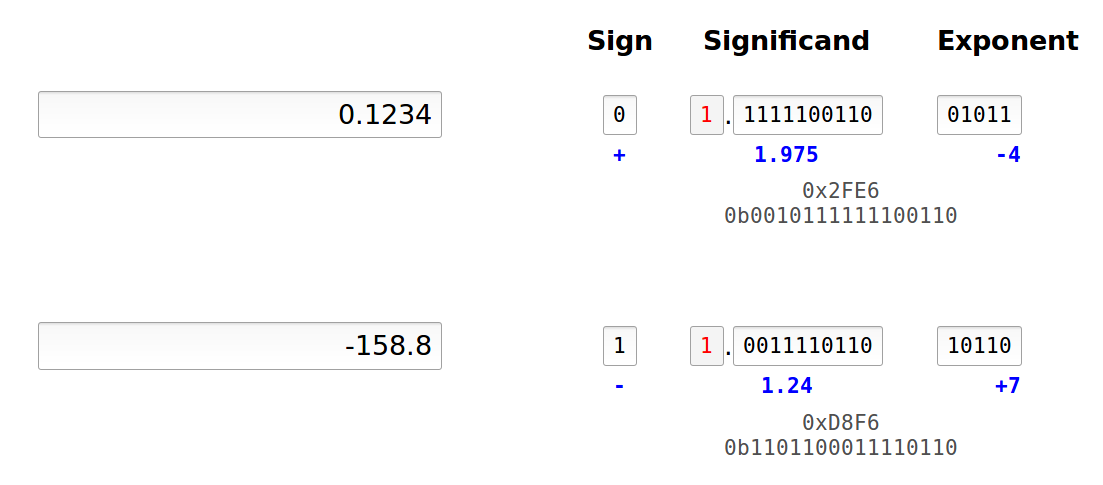
\includegraphics[height=0.45\textheight]{introduction/graphics/calculations.png}
    \end{center}
    Program do przeliczania dla różnych precyzji: \url{http://weitz.de/ieee/}
\end{frame}

\begin{frame}{Problem dużej tablicy}
    Przyjmijmy, że jesteśmy twórcą książki telefonicznej dla miasteczka, którego mieszkańcy mają
    dziwne, 10 literowe nazwiska. Aby zapewnić, że dla każdego możliwego nazwiska znajdzie się
    miejsce w naszej tablicy, musielibyśmy zapewnić jej rozmiar co najmniej 26^{10}. \\
    Jeśli w mieście żyje kilkanaście osób, zmarnujemy bardzo dużo pamięci. \\
    Na potrzeby rozwiązania skorzystajmy z 10 elementowej tablicy i funkcji skrótu znanej z numerologii.
    Zupełnie nie przejmujmy się tym, że ta funkcja ma beznadziejne własności.
    \begin{table}
        \centering
        \begin{tabular}{|c|c|c|c|c|c|c|c|c|}
            \hline
            1 & 2 & 3 & 4 & 5 & 6 & 7 & 8 & 9 \\
            \hline
            A & B & C & D & E & F & G & H & I \\
            J & K & L & M & N & O & P & Q & R \\
            S & T & U & V & W & X & Y & Z & \\
            \hline
        \end{tabular}
    \end{table}
\end{frame}
\begin{frame}{Obliczanie funkcji skrótu}
    Wartość numeryczna nazwiska KABARETKID wynosi 2121952294 $\rightarrow$ 37 $\rightarrow$ 10 $\rightarrow$ 1. \\
    MATEMATYKA $\rightarrow$ 4125412721 $\rightarrow$ 29 $\rightarrow$ 11 $\rightarrow$ 2 \\
    DELFINADDA $\rightarrow$ 4536951441 $\rightarrow$ 42 $\rightarrow$ 6 \\
    COPERNICON $\rightarrow$ 3675959365 $\rightarrow$ 58 $\rightarrow$ 13 $\rightarrow$ 4 \\
    MOCZYMORDA $\rightarrow$ 4638746941 $\rightarrow$ 52 $\rightarrow$ 7 \\
    WIBRAKACJA $\rightarrow$ 5929121311 $\rightarrow$ 34 $\rightarrow$ 7 \\
    Wartości trafiają pod odpowiednie pola tablicy, a w przypadku wystąpienia konfliktu...
    Jednym z rozwiązań jest trzymanie w tablicy wielu małych list, do których dodajemy wartości
    z kluczem o tej samej skróconej wartości. \\
    Dobra funkcja skrótu rozrzuca wartości równomiernie po całej tablicy, chociaż konflikty zawsze
    będą się zdarzały - co jest nieuniknione, gdy liczba elementów przekroczy rozmiar tablicy.
\end{frame}
\begin{frame}{Binarne drzewo poszukiwań -BST}
    \begin{center}
        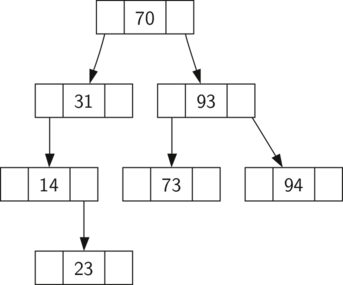
\includegraphics[height=0.8\textheight]{introduction/graphics/bst.png}
    \end{center}
\end{frame}

\begin{frame}{Notacja polska, Odwrotna notacja polska}
    Notacja polska (NP) - zapis przedrostkowy, notacja Łukasiewicza, zapis prefiksowy (prefix - przedrostek), normal Polish notation (NPN) \\
    Odwrotna notacja polska (ONP) - zapis przyrostkowy, notacja Azciweisakuł, zapis postfiksowy (postfix, sufix - przyrostek), reverse Polish notation (RPN) \\
    \begin{columns}
        \begin{column}{0.5\textwidth}
            NP:
            \[ +_1 +_2 0_1 0_2 0_3 = \]
            \[ ( 0_1 +_2 0_2 ) +_1 0_3 \]
            \[ +_1 0_1 +_2 0_2 0_3 = \]
            \[ 0_1 +_1 ( 0_2 +_2 0_3 ) \]
        \end{column}
        \begin{column}{0.5\textwidth}
            ONP:
            \[ 0_3 0_2 0_1 +_2 +_1 = \]
            \[ 0_3 +_1 ( 0_2 +_2 0_1 ) \]
            \[ 0_3 0_2 +_2 0_1 +_1 = \]
            \[ ( 0_3 +_2 0_2 ) +_1 0_1 \]
        \end{column}
    \end{columns}
    Zauważ, które działania są swoimi odbiciami lustrzanymi, a które odbiciami znaczeniowymi.
\end{frame}

\begin{frame}{Prefix, infix, postfix}
    \begin{columns}
        \begin{column}{0.3\textwidth}
            Notacja prefixowa:
            \[ +_1 0_1 0_2 = \]
            \[ +_1 +_2 0_1 0_2 0_3 = \]
            \[ +_1 0_1 +_2 0_2 0_3 = \]
            \[ +_1 +_2 +_3 0_1 0_2 0_3 0_4 = \]
            \[ +_1 +_2 0_1 +_3 0_2 0_3 0_4 = \]
            \[ +_1 +_2 0_1 0_2 +_3 0_3 0_4 = \]
            \[ +_1 0_1 +_2 +_3 0_2 0_3 0_4 = \]
            \[ +_1 0_1 +_2 0_2 +_3 0_3 0_4 = \]
        \end{column}
        \begin{column}{0.4\textwidth}
            Notacja infixowa:
            \[ 0_1 +_1 0_2 = \]
            \[ ( 0_1 +_2 0_2 ) +_1 0_3 = \]
            \[ 0_1 +_1 ( 0_2 +_2 0_3 ) = \]
            \[ ( ( 0_1 +_3 0_2 ) +_2 0_3 ) +_1 0_4 = \]
            \[ ( 0_1 +_2 ( 0_2 +_3 0_3 ) ) +_1 0_4 = \]
            \[ ( 0_1 +_2 0_2 ) +_1 ( 0_3 +_3 0_4 ) = \]
            \[ 0_1 +_1 ( ( 0_2 +_3 0_3 ) +_2 0_4 ) = \]
            \[ 0_1 +_1 ( 0_2 +_2 ( 0_3 +_3 0_4 ) ) = \]
        \end{column}
        \begin{column}{0.3\textwidth}
            Notacja postfixowa:
            \[ 0_1 0_2 +_1 = \]
            \[ 0_1 0_2 +_2 0_3 +_1 = \]
            \[ 0_1 0_2 0_3 +_2 +_1 = \]
            \[ 0_1 0_2 +_3 0_3 +_2 0_4 +_1 = \]
            \[ 0_1 0_2 0_3 +_3 +_2 0_4 +_1 = \]
            \[ 0_1 0_2 +_2 0_3 0_4 +_3 +_1 = \]
            \[ 0_1 0_2 0_3 +_3 0_4 +_2 +_1 = \]
            \[ 0_1 0_2 0_3 0_4 +_3 +_2 +_1 = \]
        \end{column}
    \end{columns}
\end{frame}

\begin{frame}{Bramki logiczne wg ANSI}
    \begin{table}
        \centering
        \begin{tabular}{|c|c|c|c|}
            \hline
            NOT & AND & OR & XOR \\
            \hline
            $\lnot$, $\sim$ & $\land$ & $\lor$ & $\veebar$ \\
            \hline
            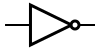
\includegraphics[width=0.25\textheight]{src/introduction/graphics/gates/NOT_ANSI.png} & 
            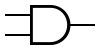
\includegraphics[width=0.25\textheight]{src/introduction/graphics/gates/AND_ANSI.png} &
            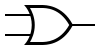
\includegraphics[width=0.25\textheight]{src/introduction/graphics/gates/OR_ANSI.png} &
            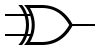
\includegraphics[width=0.25\textheight]{src/introduction/graphics/gates/XOR_ANSI.png} \\
            \hline
            \hline
            IMPLY & NAND & NOR & XNOR \\
            \hline
            $\implies$ & $\barwedge$ & $\barvee$ & $\iff$ \\
            \hline
            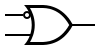
\includegraphics[width=0.25\textheight]{src/introduction/graphics/gates/IMPLY_ANSI.png} & 
            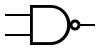
\includegraphics[width=0.25\textheight]{src/introduction/graphics/gates/NAND_ANSI.png} &
            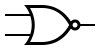
\includegraphics[width=0.25\textheight]{src/introduction/graphics/gates/NOR_ANSI.png} &
            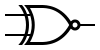
\includegraphics[width=0.25\textheight]{src/introduction/graphics/gates/XNOR_ANSI.png} \\
            \hline
        \end{tabular}
    \end{table}
\end{frame}

